\section{Beam sensor model}

If laser measurements are utilized to determine distances between the robot and obstacles, the beam sensor model can be applied. 
This model treats each beam independently and integrates various sources of error:
\begin{enumerate}
    \item \textit{Measurement Noise}: each measurement is subject to noise, which is represented using a Gaussian distribution:
        \[\Pr_{hit}(z|x,m)=\eta \dfrac{1}{\sqrt{2\pi b}}e^{-\frac{1}{2}\frac{{\left(z-z_{\text{exp}}\right)}^2}{b}}\]
        \begin{figure}[H]
            \centering
            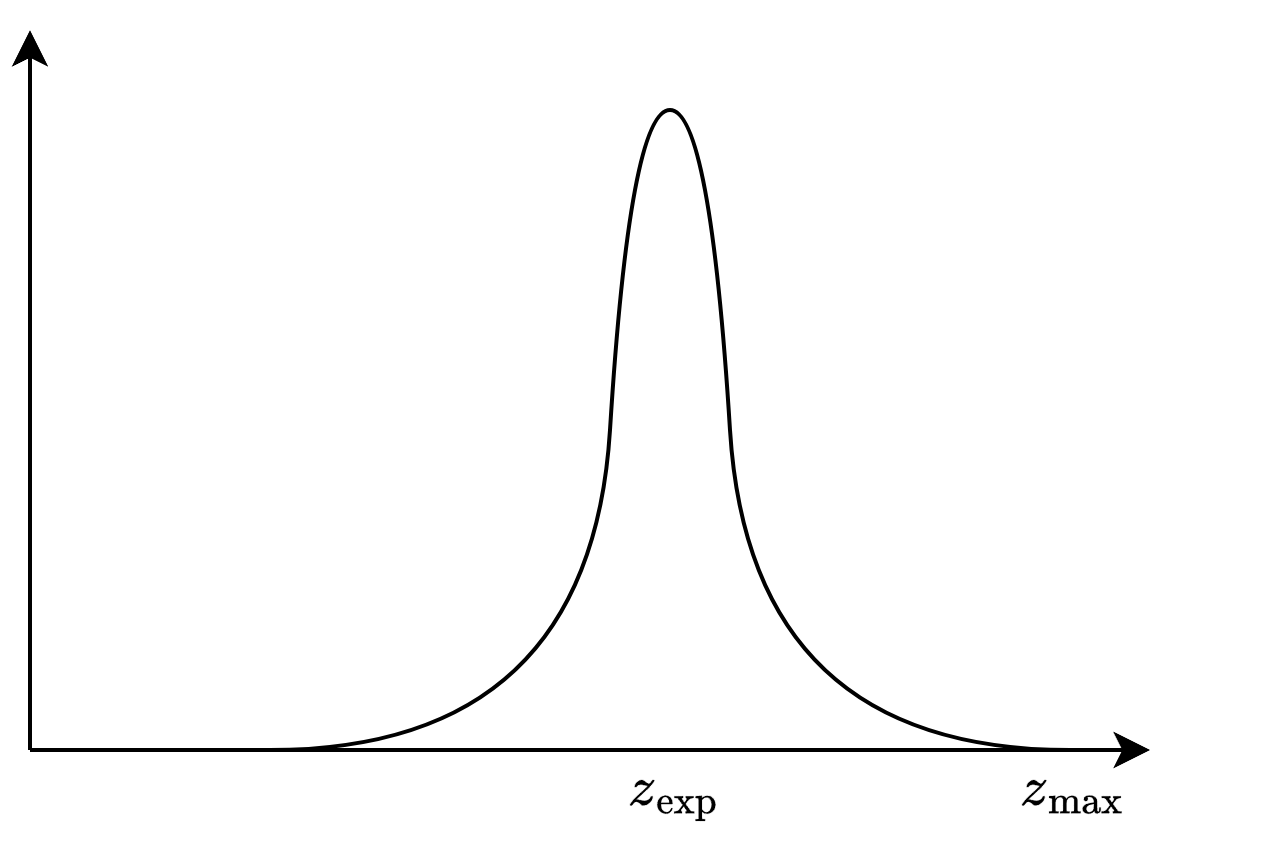
\includegraphics[width=0.4\linewidth]{images/mn.png}
            \caption{Measurement noise}
        \end{figure}
    \item \textit{Unexpected obstacles}: measurements may deviate from the actual values due to temporary obstacles obstructing the beam's path. 
        This probability is expressed as:
        \[\Pr_{\text{unexp}}(z|x,m)=\begin{cases}
            \eta\lambda e^{-\lambda z} \qquad z>z_{\text{exp}} \\
            0 \qquad\qquad\:\: \text{otherwise}
        \end{cases}\]
        \begin{figure}[H]
            \centering
            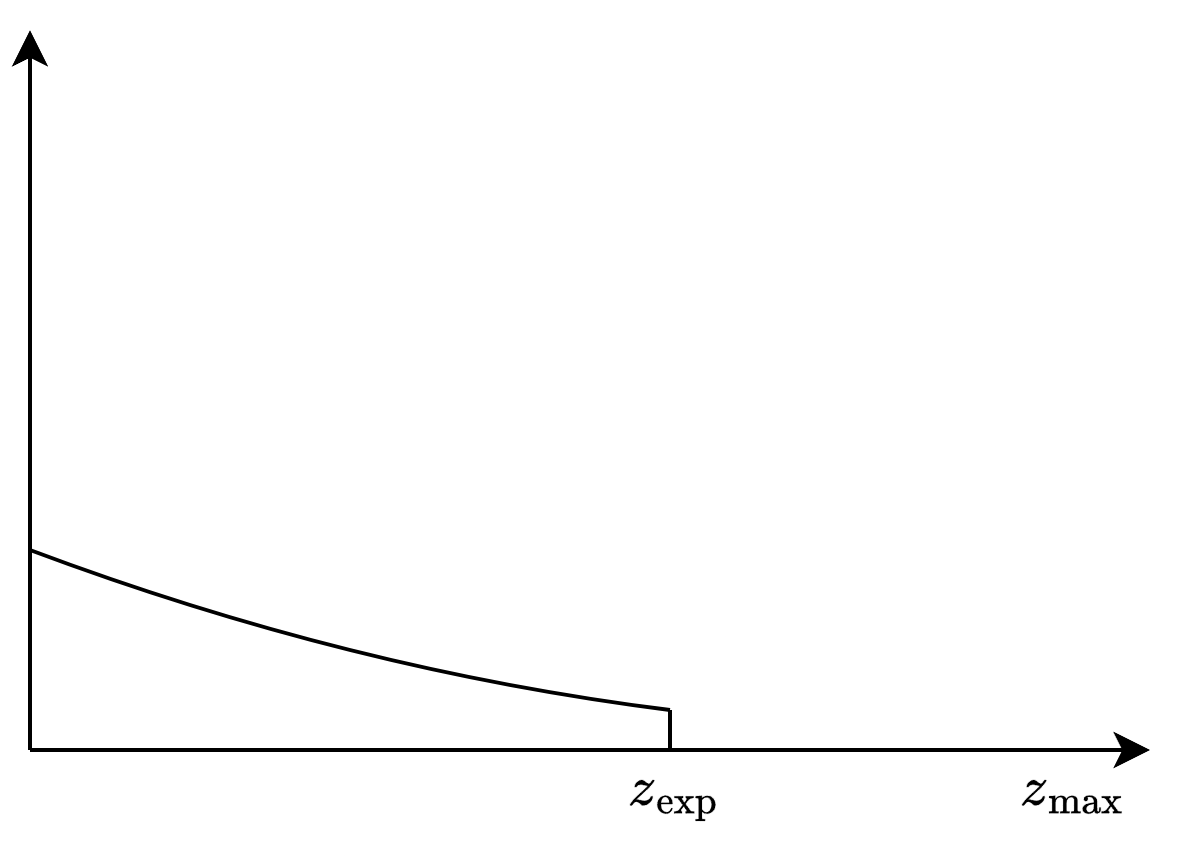
\includegraphics[width=0.4\linewidth]{images/uo.png}
            \caption{Unexpected obstacles}
        \end{figure}
    \item \textit{Random measurement}: occasionally, a completely erroneous measurement may occur with a certain probability:
        \[\Pr_{\text{rand}}(z|x,m)=\eta\dfrac{1}{z_{\max}}\]
        \begin{figure}[H]
            \centering
            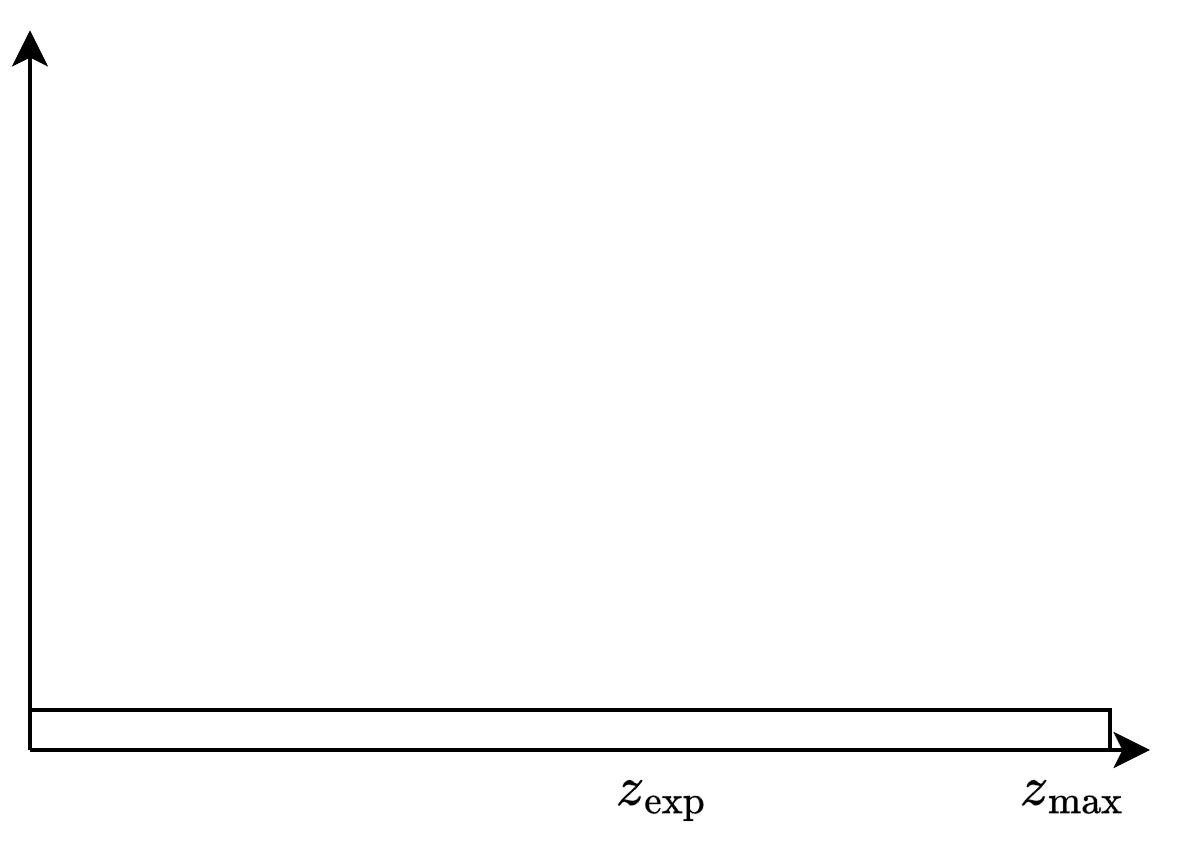
\includegraphics[width=0.4\linewidth]{images/rm.png}
            \caption{Random measurement}
        \end{figure}
    \item \textit{Maximum range}: uncertainty arises from distances beyond the sensor's reach, which is modeled as:
        \[\Pr_{\max}(z|x,m)=\eta \dfrac{1}{z_{\text{small}}}\]
        \begin{figure}[H]
            \centering
            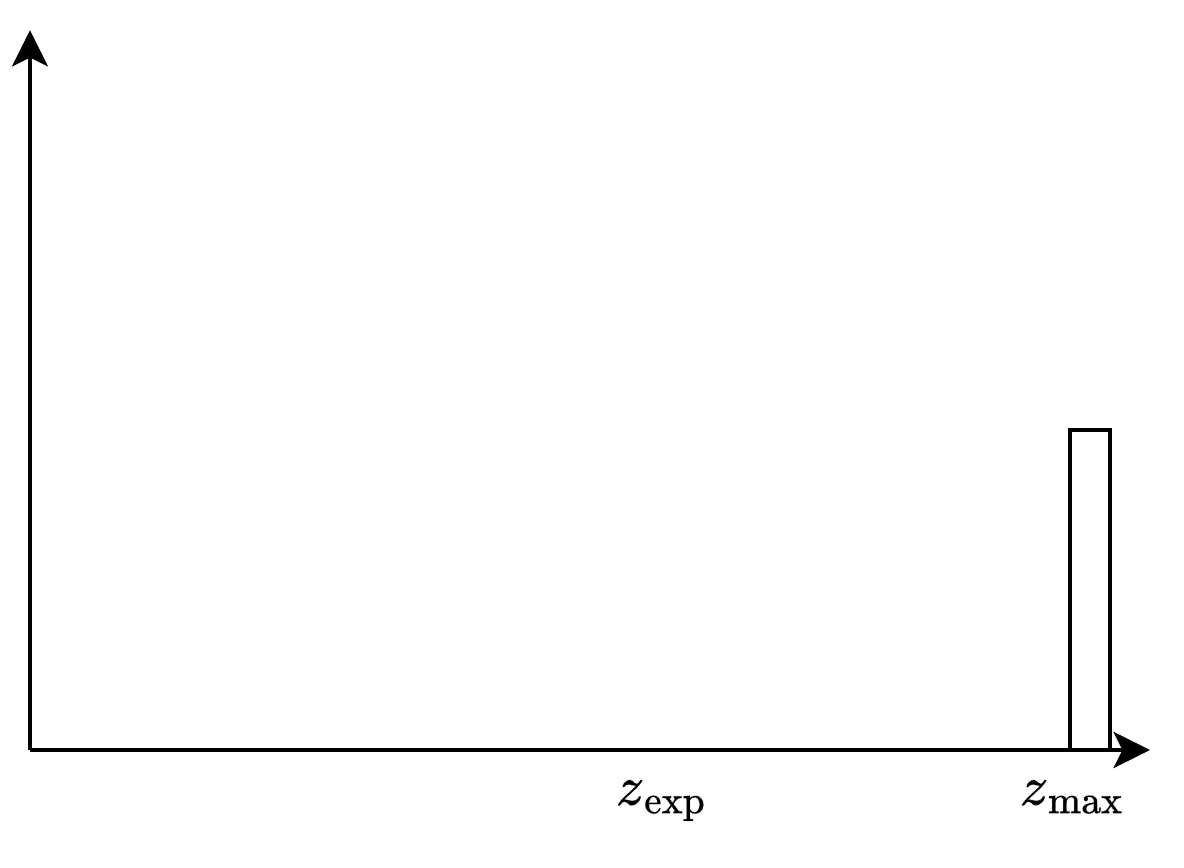
\includegraphics[width=0.4\linewidth]{images/mr.png}
            \caption{Random measurement}
        \end{figure}
\end{enumerate}
The total probability can be computed by combining these individual probabilities:
\[\Pr(z|x,m)=\begin{bmatrix}
    \alpha_{\text{hit}} \\
    \alpha_{\text{unexp}} \\
    \alpha_{\text{max}} \\
    \alpha_{\text{rand}}
\end{bmatrix}^T \cdot \begin{bmatrix}
    \Pr_{\text{hit}}(z|x,m) \\
    \Pr_{\text{unexp}}(z|x,m) \\
    \Pr_{\text{max}}(z|x,m) \\
    \Pr_{\text{rand}}(z|x,m)
\end{bmatrix}\]
The overall structure of this probability distribution is depicted as follows:
\begin{figure}[H]
    \centering
    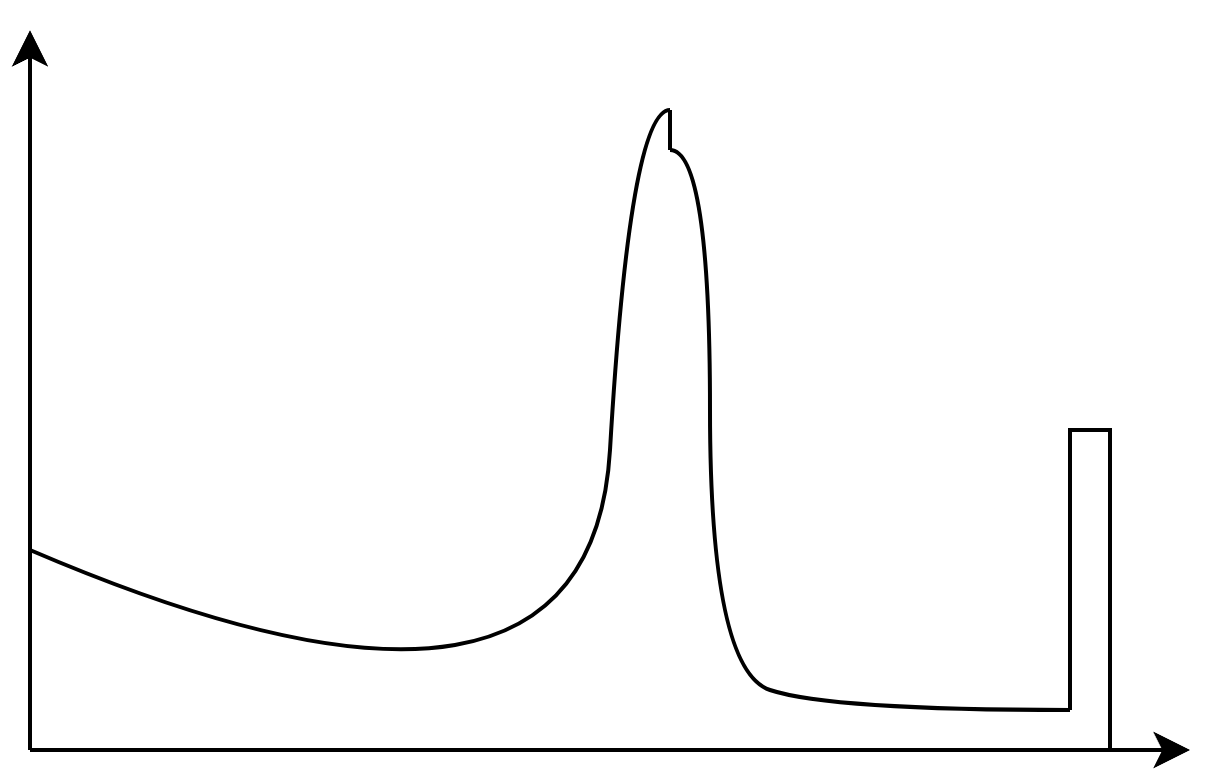
\includegraphics[width=0.6\linewidth]{images/bsm.png}
    \caption{Probability distribution of beam sensor model}
\end{figure}

\subsection{Calibration}
To calibrate the sensor, we can collect data at specific distances, such as 300 cm and 400 cm, and then estimate the model parameters using maximum likelihood $\Pr(z|z_{\text{exp}})$.
Since it's impractical to calibrate the sensor for every possible distance, we typically select a few representative distances and interpolate or use a mean for the missing data.
\begin{figure}[H]
    \centering
    \begin{subfigure}{0.49\textwidth}
        \centering
        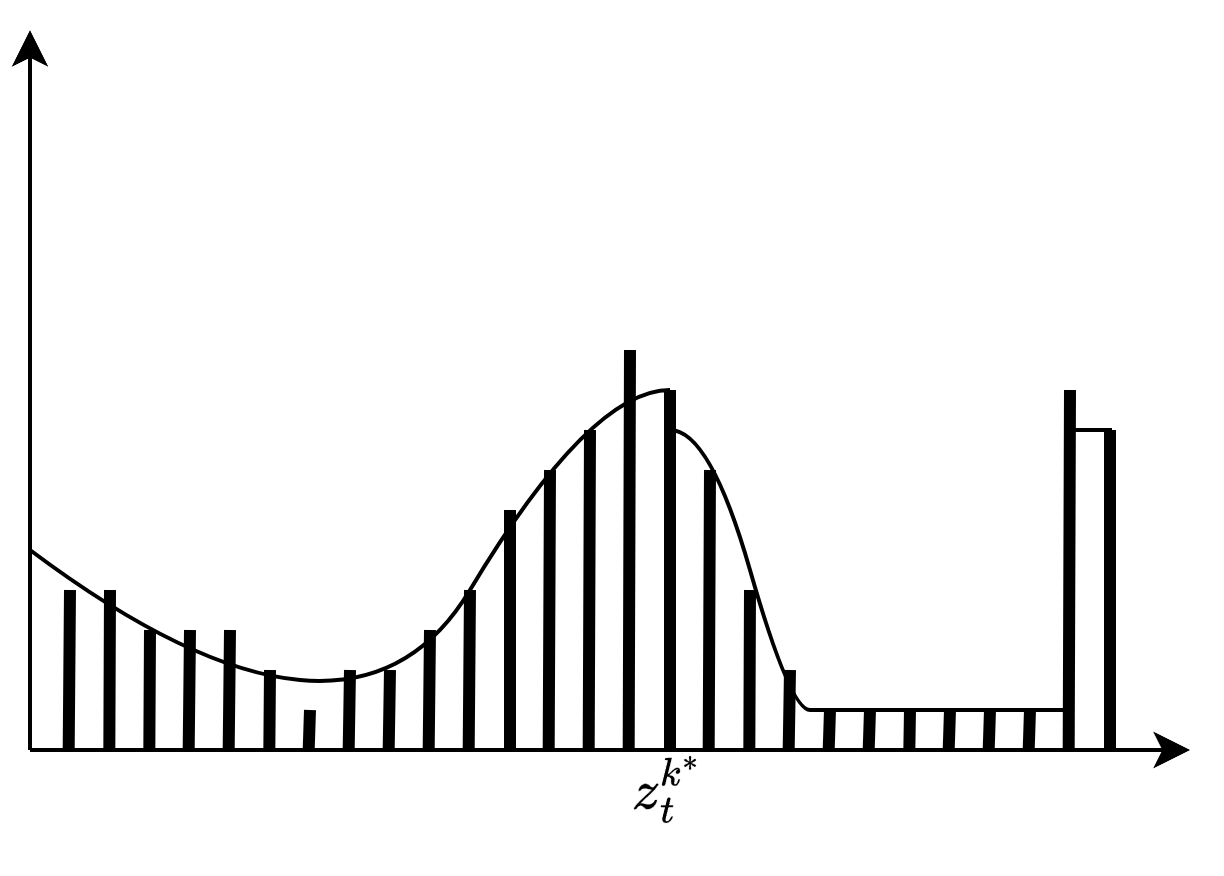
\includegraphics[width=0.75\linewidth]{images/sonarcalib.png} 
        \caption{Sonar}
    \end{subfigure}
    \begin{subfigure}{0.49\textwidth}
        \centering
        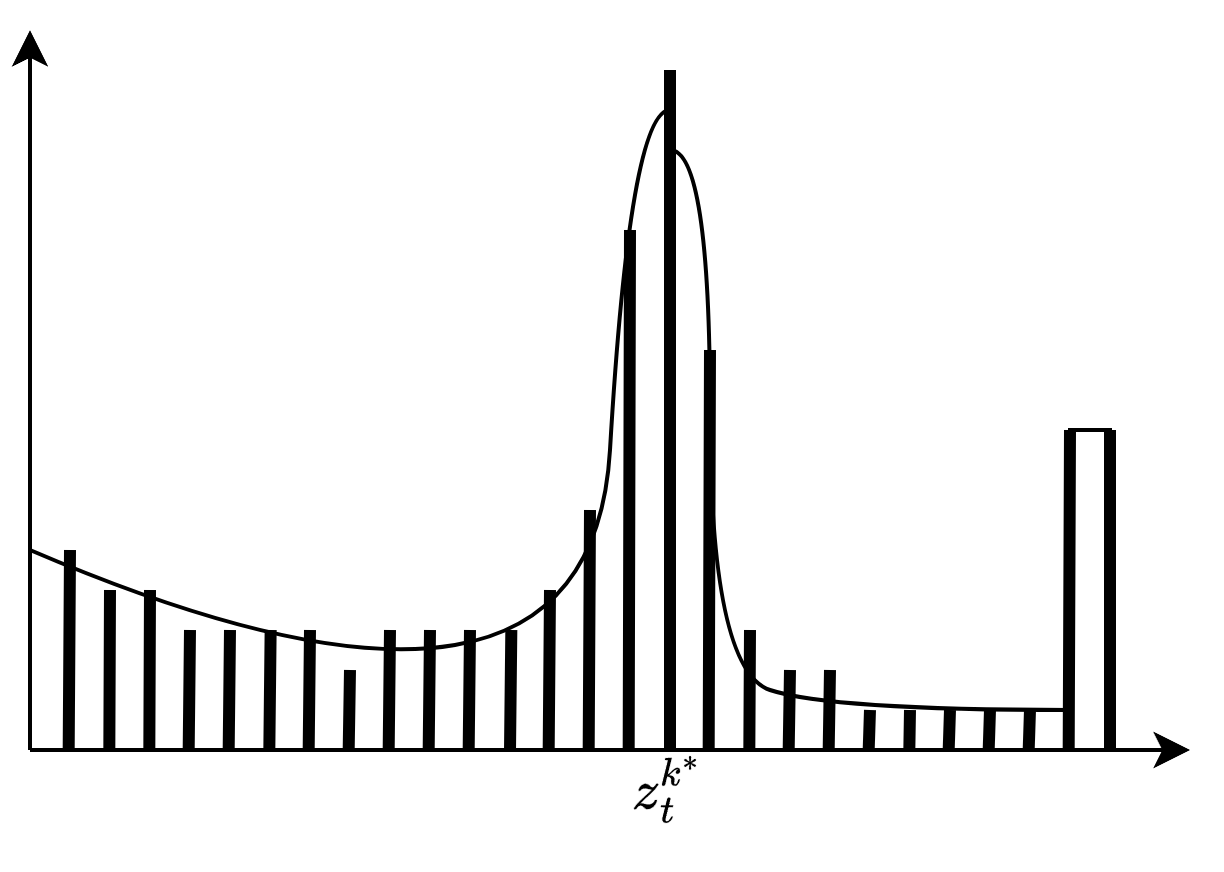
\includegraphics[width=0.75\linewidth]{images/lasercalib.png}
        \caption{Laser}
    \end{subfigure}
    \caption{Calibration at three hundreds centimeters}
\end{figure}
By acquiring data at these distances, we can estimate the parameters of the sensor model to improve its accuracy across a range of distances.

\subsection{Model likelihood}
In this model, our objective is not to find the most likely position given the measurements, but rather to determine the position that maximizes the likelihood of the sensor readings.
Therefore, in this context, we are searching for a position $x$ such that the measurements from the sensors are maximized. 
This approach focuses on identifying the position that aligns best with the observed sensor data, rather than estimating the robot's actual position.